\documentclass{article}
\usepackage{amsmath,amssymb,tikz,mathrsfs}
\usetikzlibrary{calc,intersections,backgrounds}
\usepackage[margin=3.5cm]{geometry}
\usepackage[UTF8,space]{ctex}
\usepackage[thmmarks]{ntheorem}
\newtheorem{Definition}{定义}[section]
\newtheorem{Theorem}[Definition]{定理}
\newtheorem{Lemma}{引理}
\newtheorem{Guess}{猜想}[section]
\newtheorem{Proposition}{命题}[section]
\newtheorem{Deduction}[Proposition]{推论}
\theoremstyle{nonumberplain}\theorembodyfont{\normalfont}\theoremsymbol{$\Box$}
\newtheorem{Proof}{证:}
\begin{document}
\section{三角函数}
  \begin{Theorem}
    三角方程 $a\sin x + b\cos x=c$ 有解的充要条件是 $a^2+b^2\ge c^2$.
  \end{Theorem}
  \begin{Proof}
    原方程可化为
     \[ \frac{a}{\sqrt{a^2+b^2}}\sin x +\frac{b}{\sqrt{a^2+b^2}}\cos x=c\].\par
    即$sin(x+\phi)=\dfrac{c}{a^2+b^2}$ (其中$\phi$角所在象限由 $a,b$ 的符号确定 , $\phi$ 的值由 $\tan\phi=b/a$ 确定)。\par
    因为 $|sin(x+\phi)|\le1$ , 所以 $\bigg|\dfrac{c}{a^2+b^2}\bigg|<1$, 即 $a^2+b^2\ge c^2$.\par
    显然 , 其逆命题也真 
  \end{Proof}
   
\section{$\sqrt2$是一个无理数}
  古希腊数学家曾认为一切数皆整数之比,直到他们发现$\sqrt2$这个反例。这个事实用今天的话说$\sqrt2$是一个十数无理数,用欧几里得的话说 1 和$\sqrt2$是不可公约的。实际上欧几里得会说正方形的边长和对角线是不可公约的。\par

\begin{tikzpicture}[scale=.8,background rectangle/.style=
{draw=blue!50,fill=blue!20,rounded corners=1ex},show background rectangle]
\node[above right]at(0,2.5){\large\textbf{为什么说正方形的边长是$\sqrt2$?}};
\draw(3,0)rectangle+(2,2) (3,0)--+(2,2);
\node[below] at(3,0){1};
\node[right] at(5,1){1};
\node[below]at(4,1){$\sqrt2$};
\node[below right]at(0,2){\parbox{2cm}{(1)由勾股定理,单位正方形的对角线的平方为 2}};

\draw (11,1)rectangle+(2,2) (11,1)--+(2,2)--+(4,0)--+(2,-2)--cycle;
\draw[dotted](13,-1)--+(0,2)--+(2,2);
\node[above]at(12,2){$\sqrt2$};
\node[right]at(13,2){1};
\node[below right]at(6,2){\parbox{3cm}{(2)根据图中面积关系,亦知单位正方形的面积是以对角线为边长的面积的 $1/4$}};
\end{tikzpicture}

可公约以及不可公约都是针对两条线段来说的。设$a,b$是两条线段,$a$不长于$b$,我们用$a$来量$b$,一段一段地量,如果剩下一小段的话,再用这一小段量$a$,这个过程可以一直进行下去,如果有那么一刻,刚好量完不剩下,就说$a,b$是可公约的,否则就说$a,b$是不可公约的。
\par为什么$1$和$\sqrt2$不可公约呢?
\par
\begin{minipage}{\textwidth}\begin{minipage}{0.6\textwidth}
如右图,取$BE=BC$,作$EF\perp BD$交$CD$于$F$,则$DE=EF=FC$(可能不是很显然)。$BC$量$BD$之剩余为$ED$,以$ED$量$BC$同样是以正方形的边长量对角线,无穷无尽。所以正方形的边长与对角线不可公约。
\end{minipage}\quad\begin{minipage}{0.4\textwidth}
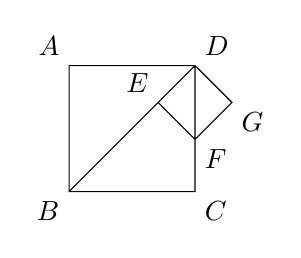
\begin{tikzpicture}[scale=.8]
\coordinate[label=above left:$A$](A)at(0,2);
\coordinate[label=below left:$B$](B)at(0,0);
\coordinate[label=below right:$C$](C)at(2,0);
\coordinate[label=above right:$D$](D)at(2,2);
\coordinate[label=above left:$E$](E)at($(B)!1!45:(C)$);
\coordinate[label=below right:$F$](F)at($(E)!1!-90:(D)$);
\coordinate[label=below right:$G$](G)at($(D)!1!90:(E)$);
\draw (B)rectangle(D) (B)--(D) (E)--(F)--(G)--(D);
\end{tikzpicture}\end{minipage}\end{minipage}

\newcommand\proof[1]{\par\vspace*{1em}{\large\bf#1}\par}
\proof{证明$\mathbf{\sqrt2}$是无理数之整除}
反设$\sqrt2=q/p$(既约),则$q^2=2p^2$, $\Rightarrow 2|q \Rightarrow 4|2p^2 \Rightarrow 2|p$,与$q/p$既约矛盾。

\proof{3 进制表示}
设$x=q^2=2p^2$,以 3 进制表示$x$,由于平方数只以 0 或 1 结尾,而平方数的 2 倍只以 0 或 2 结尾,所以$x$以 0 结尾。

\proof{算术基本定理}
把$x$质因数分解,$x=q^2$表明有偶数个 2,$x=2p^2$表明有奇数个 2,矛盾。

\proof{平方为整数}
$2=q^2/p^2$为一整数,所以$p^2|q^2$与$p,q$既约矛盾。

\proof{取出小数部分}
$\sqrt2=q/p$ $\Rightarrow 2q/p=p/q$ $\Rightarrow \{2q/p\}=\{p/q\}$ $\Rightarrow a/p=b/q$ $\Rightarrow \sqrt2=b/a$无穷递归,引发矛盾。

\proof{又一个无穷递归}
$q^2=2p^2 \Rightarrow (2p-q)^2=2(q-p)^2$.

\proof{图形上的无穷递归}
\begin{minipage}{\textwidth}\begin{minipage}{0.6\textwidth}
把边长为$p$的正方形按如图所示的方式放在边长为$q$的正方形内,重合部分的面积等于空白部分的面积,若$q^2=2p^2$,必有$b^2=2a^2$,无穷递归。
\end{minipage}\quad\begin{minipage}{0.4\textwidth}
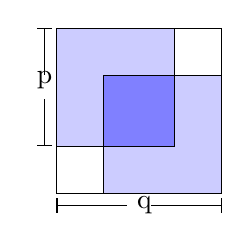
\begin{tikzpicture}[scale=.3]
\draw (0,0)rectangle(7,7);
\filldraw[fill=blue!20](0,2)rectangle(5,7);
\filldraw[fill=blue!20](2,0)rectangle(7,5);
\filldraw[fill=blue!50](2,2)rectangle(5,5);
\draw[|-](-.5,2)--(-.5,4)node[above=0pt]{p};
\draw[|-] (-.5,7)--(-.5,5);
\draw[|-](0,-.5)--(3,-.5)node[right=0pt]{q};
\draw[|-] (7,-.5)--(4,-.5);
\end{tikzpicture}\end{minipage}\end{minipage}

\proof{运用极限}
\def\Crm{\mathrm{C}}\def\Zbf{\mathbf{Z}}
$\sqrt2=q/p \Rightarrow (\sqrt2)^np$总是整数,但$0<(\sqrt2-1)^np=\displaystyle\sum_{k=0}^n\big[\Crm_n^k(\sqrt2)^k(-1)^{n-k}p\big]\in\Zbf$,与$\displaystyle\lim_{n\to\infty}(\sqrt2-1)^np=0$矛盾。

\proof{连分数}
由于$1/(\sqrt2-1)=\sqrt2+1$,知化为连分数是无限长的,所以$\sqrt2$是无理数。

\proof{整系数多项式}
$\sqrt2$为方程$x^2-2=0$的根,由整系数多项式有理根的性质,$\sqrt2$为一无理数。

\proof{艾森斯坦判别法}
$x^2-2=0$在有理数域上不可约,所以$\sqrt2$是无理数。


\section{无以言表的大数}
\subsection{引子}
小时候,我们一个一个地学习数字。先学会 1, 然后是 2, 再然后是 3. 那时候,我们甚至数不清自己有多少根手指头。渐渐地,我们可以数到 10, 数到 20, 后来可以数到 100. 之后就不同了,我们竟然顿悟计数原理,不仅可以轻易地数到 1000, 而且认为可以数到 1 万,甚至 1 亿。只要我愿意数,那只是时间的问题。

这时候,我们觉得认识了所有的数,并且可以写出任意大的数,需要做的仅仅是先写个 1, 然后在后面不断地添 0. 学习了“幂”之后,就连宇宙间的粒子数也仅需写下$10^100$就远远超过了它。但是你相信数学中的大数还可以大得让你无以言表吗?

\subsection{古德斯坦数}
正如十进制数 1206 可以写成 $1\times10^3+2\times10^2+6$一样,四进制数$102312$可以写成$1\times4^5+2\times4^3+3\times4^2+1\times4+2$. 然而不完美的是$4^5$中的 5 并不是一个四进制数,而应换成$4+1$, 这才是“真正的”四进制展开。同理,二进制数 1000011 写成$2^6+2+1$还不够,$2^{2^2+2}+2+1$ 才是它真正的二进制展开。

所谓的古德斯坦数列$G_i{m}$是由初始正整数$m$生成的,其中$G_1^m=m$, $G_k^m$是把$G_{k-1}^m$的完全$k$进制展开式中所有数字$k$都替换成$k+1$后所得到的数再减 1. 比如:
\begin{align*}
G_1(8)&=8=2^{2+1}\\
G_2(8)&=3^{3+1}-1=80=2\times3^3+2\times3^2+2\times3+2\\
G_3(8)&=2\times4^4+2\times4^2+2\times4+2-1=533=\cdots\\
G_4(8)&=\cdots\\
\end{align*}

古德斯坦定理指出,不管初始数$m$是多少,按照上述方法迭代下去,最后总有一个时刻会变为 0. 

例如$m=3$时,6 步之后数列便变为了 0.
\begin{align*}
G_1(3)&=2+1\\
G_2(3)&=3+1-1=3\\
G_3(3)&=4-1=3\\
G_4(3)&=3-1=2\\
G_5(3)&=2-1=1\\
G_6(3)&=1-1=0\\
\end{align*}

但是当$m=4$时,情况就不大一样。它会持续增长到几百,几万,几亿,然后增长到几百位,几千位,甚至上亿位。根据古德斯坦定理,它最终还是会变为 0,只是这个过程可能极长。事实上,一直到$3\times2^{402653211}-2$步数列才会变成 0. 
\begin{align*}
G_1(4)&=2^2\\
G_2(4)&=3^3-1=26=2\times3^2+2\times3+2\\
G_3(4)&=2\times4^2+2\times4+1\\
G_4(4)&=2\times5^2+2\times5\\
G_5(4)&=2\times6^2+2\times6-1=83=2\times6^2+6+5\\
\cdots
\end{align*}

\newcommand\Gscr[1]{$\mathscr G(#1)$}
采用\Gscr m 表示初始值为$m$时迭代到 0 所需要的步数。\Gscr m 增长速度如此之快,\Gscr3$=6$很小,\Gscr4$=3\times2^{402653211}-2$, 位数上亿,而\Gscr5则更大,它的位数都将远远超过\Gscr4, 而\Gscr8呢?即使说它有多少位,或者位数有多少位,或者在前面那句话里嵌套进多少个“的位数”也无法表达出它的大小来。

除非我们创造更大的大数表示法。

\subsection{超级幂}
加法之后是乘法,乘法之后是乘方,乘方之后呢?加、乘、幂方分别为第一、第二、第三级运算,有没有和第四级运算呢?不难想到要把幂重叠起来:
$$\LARGE a^{a^a}$$
构成一个超级幂。

我们约定它的意义是$a^{(a^a)}$, 因为较之$(a^a)^a$,前者更能体现“大”这一字眼。请看:
  \begin{align*}
  &(2^2)^2=4^2=16\\
  &2^{2^2}=4^2=16\\
  \end{align*}
莫急
  \begin{align*}
  &(3^3)^3=27^3=19683\\
  &3^{3^3}=3^27=7625597484987
  \end{align*}
差距出来了
  \begin{align*}
  &(10^10)^10&=10^{100}\quad \text{拥有100个0}\\
  &10^{10^10} \quad \text{却拥有100亿个0}
  \end{align*}
巨大的差距令人颇为满意。
\def\sc{\scriptstyle}
$${}^ba=a^{a^{\sc\cdot^{\sc\cdot^{\sc\cdot^{\sc a}}}}}\bigg\}b\text{个}a$$
称为超级幂。这就是乘方之后的第四级运算。

不妨想一下,${}^32=16$, ${}^42=65536$, ${}^52$将拥万位,那么${}^26$就更大了。${}^310$已拥百亿位,那么${}^{10}10$呢?${}^{100}100$呢?

在我们书写诸如${}^{10}10$这样的超级幂的时候,我们的困惑也随之而来。以前,我们苦恼于知道的数不够数身边的物体,现在,我们苦恼于身边的物体不够计数。于是问道,超级幂有什么用吗?

实际上,数学中的数不必存在于现实中,它只需要存在于我们的想象中。人类虽然渺小,惟想象可以超越整个宇宙。或许今天我们难以想象的大数,未来的人会习以为常,反倒为我们对超级幂感到无可适从而吃惊不已。

\subsection{第$n$级运算}
有了第四级运算,我们自然会想,有没有第五级运算呢?有没有更高级的运算呢?
\par $$\begin{tikzpicture}[scale=.5]
\draw(0,1.2)node{$\sc a$}(1,0.2)node{$\sc  a$};
\fill (.25,.95)circle(1pt) (.5,.7)circle(1pt) (.75,.45)circle(1pt);
\end{tikzpicture}  \!\! a \bigg\}\ b\text{个}a=?$$

古德斯坦的厉害之处就在于它定义了记号$G(n,a,b)$用于表示$a$和$b$的第$n$级运算。

当$n=0$时,规定$G(0,a,b)=b+1$;
递归定义$G(n,a,b)=G(n-1,a,G(n,a,b-1))$. 补充定义$G(1,a,0)=a$, $G(2,a,0)=0$, $G(3,a,0)=G(4,a,0)=\cdots=1$.

例如$G(1,3,2)=G(0,3,G(1,3,1))=G(1,3,1)+1=G(1,3,0)+2=3+2$
实现加法。

又如$G(2,a,b)=G(1,a,G(2,a,b-1))=a+G(2,a,b-1)=a\times b$实现乘法. 

再比如
\begin{align*}
&G(5,5,5)=G(4,5,G(5,5,4))={}^{G(5,5,4)}5\\
&G(5,5,4)=G(4,5,G(5,5,3))={}^{G(5,5,3)}5\\
&G(5,5,3)=G(4,5,G(5,5,2))={}^{G(5,5,2)}5\\
&G(5,5,2)=G(4,5,G(5,5,1))={}^{G(5,5,1)}5\\
&G(5,5,1)=G(4,5,G(5,5,0))=5\\
\end{align*}
\def\ssc{\scriptscriptstyle}
于是$G(5,5,2)={}^55$, $G(5,5,3)=\raisebox{1ex}{$\sc{}^55$}5$, $\cdots$, $G(5,5,5)=\raisebox{12pt}{$\ssc5$}\raisebox{9pt}{$\ssc5$}\raisebox{6pt}{$\ssc5$}\raisebox{3pt}{$\sc5$}5$

这样就形式化地给出了第$n$级运算。

很多外文论谈使用$a[n]b$来表示$G(n,a,b)$. 当然,有$a[n]b$就有$a[a[n]b]$, 从而有$a[a[a[n]b]b]b$, $\cdots$ 没有最大的数,只有更大的数。

然而在无限那里,再大的数都不算大。正如在永恒那里,再长的时间都只能像 1 秒那样一闪而过。但是在飞跃到无限之前,你能想像的最大的数有多大,就看你的本事了。


\section{无穷集合}
\begin{quote}
没有任何问题可以像无穷那样深深地触动人的情感,很少有别的观念无穷那样激励理智产生富有成果的思想,然而也没有任何其它的概念能像无穷那样需要加以阐明。
\end{quote}
无穷,我们希望站在数学的角度从各个方面认识它。最具引力的就是无穷集合,据说它把康托吸引进了精神病医院,足见其诡异与魅力。它是数不尽的,取一个,再一个,第三个,第四个$\cdots\cdots$ 永远取不尽,自然数集就是这样的。因此采用“有一个子集一一对应到自然数集的集合叫做无穷集合”作为定义。至此,无穷不仅仅是有穷的否定了。但是上述定义由于借用了自然数集这个无穷集,因而不是彻底地,不若径用自然数集的一个性质---可以与其真子集一一对应---来定义无穷集合。下面证明它们是等价的,先从前者推后者,后逆之。
\footnote{无限!再也没有其他问题如此深刻地打动过人类的心灵。---希尔伯特}

(1)让对等于自然数集的元素对应到后接元,其余元素对应到自身得所需,由于第一个元素被剩下,就证明了我们所想要的结果。

(2)若$A_1$是$A$的真子集,$f$是$A_1$到$A$的一一映射,取$x_1\in A_1$但$X_1\not\in A$,令$x_2=f(x_1), x_3=f(x_2),x_4=f(x_3),\cdots$. 首先$x_1$与$x_2,x_3,\cdots$皆不相同,然后从原像$x_1,x_2,\cdots,x_k$互不相同知像$x_2,x_3,\cdots,x_{k+1}$互不相同,因而$x_1,x_2,\cdots,x_{k+1}$互不相同。由归纳原理,$x_1,x_2,x_3,\cdots$互不相同,让它对等到\textbf{N}, 功成。
\par\vspace{1em}

虽然一个是另一个的一部分,但是就数目而言,如果仔细思索的话,它们是相同的。请为此惊奇:在永恒面前,年与日不分;在无限那里,步与里无别!

转,1 后面有 2,2 后面有 3,$\cdots\cdots$ 继之不止,则自然数无穷;一分为二,二分为四,$\cdots\cdots$ 永不可尽,则线段上的点无穷。虽然元素不可穷尽,但是我们确信彼二者可以从整体上把握,也就是说它们是集合。如果不承认这一点,关于无穷就几乎什么也没有。现在这些无限的东西本身是一个实体,就像我们的双手那样亲切。而且,现今所谓认知无穷就是认知彼二者。

回,还要惊奇了。无穷集合对等到它的部分,这是极为平常的。所以惊奇者,叙述与思考的方式不平常而已。在事实面前,这是微不足道的。

两个集合如果可以对等就说势相同。凭这句话不去叙述“势”这个概念,我也没有能力说清楚。与自然数集等势的集称为可数集。整数集是可数的,下面证明有理数集及代数数集也是可数的。\marginpar{什么,不证明一下整数集是可数的吗?}

先证可数个可数集之并是可数的。如图,依法让有序自然数对排成一列就建立起$\mathbf{N}\times\mathbf{N}\to\mathbf{N}$的一一映射。我们甚至可以把对应关系写出来:
$$f(x,y)=\frac12(x+y)(x+y+1)+x$$

(1)在上面做一些增减工作就可以把有理数排成一列了.\marginpar{任给一个有理数,尽管可能很靠后,我们总能在这个序列中找到它。}

(2)注意对$\forall n\in \mathbf{Z}$, $a$是有理数当且仅当$a+n$是有理数,而数轴上这样的敬意的个数是可数的。

(1)代数数是数多项式的复根。把整系数多项式按系数绝对值的和分类,有可数个类,第一类有有限个多项式,每个多项式的根的个数至多等于它的次数,因此代数数集是可数的。

(2)考虑到$n$次多项式可由$n$元数组决定,这是可数的,\marginpar{不是只证明了2元自然数组是可数的吗?}因此,$n$次多项式的根是可数的。次数仅取自然数,可数个可数集之并是可数的。

哦!你可能难以理解,反正我是疯掉了。但是当我明白之后,又变得激动不已了。直线上的有理数不是稠密的吗,任意两个有理数之间不是还有另一个有理数吗,为什么它会和比教授的头发还稀疏的自然数对等呢?大概这就是无穷集合的不可思议之处吧。

我们常用下述定理,它简化思考的表达。下面的证明为了显现思路,放弃了一些细节。$|A|$表示集合$A$的势,$|A|\le|B|$是说存在$A$到$B$的单射,又若不存在$A$到$B$的双射,则记作$|A|<|B|$. 

Bernstein定理:$|A|\le|B|$且$|B|\le|A|$蕴含$|A|=|B|$.\marginpar{干嘛把这个定理写这么抽象,不知道哥不喜欢翻译吗?}
证:不断使用$A$到$B$的单射及$B$到$A$的单射,$A$映到$B_1$时,$A_1$被映到$B_2$(含于$B_1$); \marginpar{即使为了简洁,也不能连$B_1$是$A$到$B$的那个单射中的像集,$A_1$是$B$到$A$的那个单射中的像集也不说一声吧?}$B$映到$A_1$时,$B_1$被映到$A_2$(含于$A_1$); $A_1$映到$B_2$时,$A_2$被映到$B_3$(含于$B_2$),$\cdots$ 示意其一一映射如下:


$A,B$中的元素,要么出现在某个差集中,要么永远在$A_k,B_k(k=1,2,\cdots)$中,对于前者,对应已经建立如上,记后者的全体为$C_1$和$C_2$当$A$映到$B_1$时,必有$C_1\to C_2$在这个映射下为双射,首先$C_1$中元素的像必在$C_2$中,否则$a_1\to a_2$, $a_2\not\in C_2$, 存在$k$使$a_2\not\in B_k$, 但$A_{k-1}$对等于$B_k$, $a_1$却无象可对,矛盾。同理,$C_2$中元素的原像必在$C_1$中。至此建立了$A$到$B$的双射。

上面的$C_1,C_2$可能是空集,这是很奇怪的事,举一个这样奇怪的例子。设$A_1$是正整数集,$A_2=\{2,4,\cdots,2k,\cdots\}$, $\cdots$ $A_n=\{2^n,2\cdot2^n,\cdots,k\cdot2^n,\cdots\}$, $\cdots$ 于是$A_1\supset A_2\supset A_3\cdots$且$A_1\approx A_2\approx A_3\approx\cdots$(对等),但是$\varnothing=A_1\cap A_2\cap A_3\cap\cdots$.

$$\frac2\pi=\frac{\sqrt2}2\times\frac{\sqrt{2+\sqrt2}}2\times
\frac{\sqrt{2+\sqrt{2+\sqrt2}}}2\times\cdots
~~\hbox{(韦达1593)}$$
$$\frac\pi2=\frac{2\times2}{1\times3}\times\frac{4\times4}{3\times5}
\times\frac{6\times6}{5\times7}\times\cdots~~\hbox{(沃利斯1650)}$$

$$\frac\pi4=4\arctan\frac15-\arctan\frac1{239}~~\hbox{(Martinl1706)}$$

$$\frac\pi4=1-\frac13+\frac15-\frac17+\frac19-\cdots~~\hbox{(Leibniz)}$$

$$\frac\pi4=\frac12-\frac1{3\times2^3}+\frac1{5\times2^5}-
\frac1{7\times{2^7}}+\cdots~~\hbox{(Euler)}$$

$$\frac4\pi=1+\cfrac1{2+\cfrac9{2+\cfrac{25}{2+\cfrac{49}{2+\cdots}}}}~~\hbox{(BrownCouro)}$$

$$\frac\pi6=\frac12+\frac1{2\times3\times2^3}+
\frac{1\times3}{2\times4\times5\times2^5}+\frac{1\times3\times5}
{2\times4\times6\times7\times2^7}+\cdots~~\hbox{(Newton)}$$

$$\frac\pi4=3\arctan\frac14+\arctan\frac5{99}~~\hbox{(Herdon)}$$

$$\sqrt\pi=\int_{-\infty}^\infty e^{-x^2}dx$$

$$\frac{\pi^2}6=1+\frac1{2^2}+\frac1{3^2}+\frac1{4^2}+\cdots~~\hbox{(Euler)}$$

$$\pi=\frac{426880\sqrt{10005}}{\sum_{n=0}^\infty\displaystyle\frac{(6n)!\,
(545140134n+13591409)}{(n!)^3(3n)!\,(-640320)^{3n}}}~~\hbox{(Chudnovsky)}$$
\end{document}
